\documentclass{article}
\usepackage{hyperref}
\usepackage{amsmath}
\usepackage{amssymb}
\usepackage{pgfplots}
\usepackage{float}
\usepackage{todonotes}
\usepackage{tikz}
\usepackage[shortlabels]{enumitem}

\renewcommand{\Re}{\mathbb{R}}
\newcommand{\Li}{\mathcal{L}}
\newcommand{\Ex}{\mathbb{E}}
\renewcommand{\Pr}{\mathbb{P}}
\newcommand{\Hy}{\mathcal{H}}
\newcommand{\sign}{\text{sign}}
\newcommand{\error}{\text{error}}

\newcommand\bigO[1]{
    \ensuremath{\mathcal{O}\left(#1\right)}
    }

\newcommand{\sigmoidPlot}{
    
    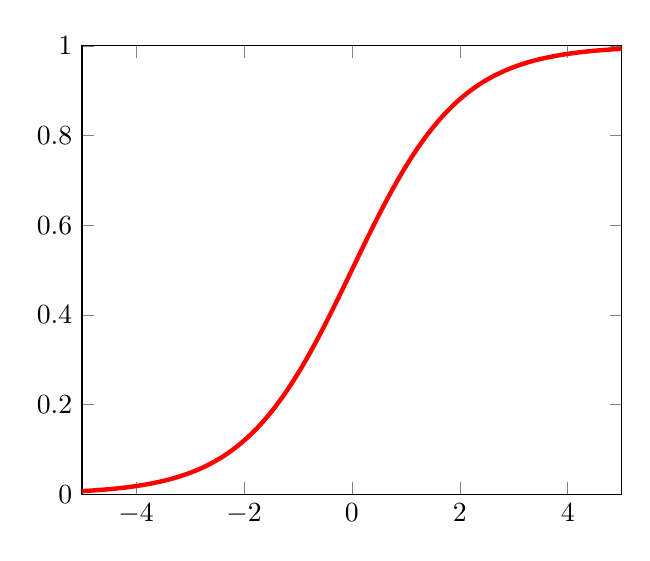
\begin{tikzpicture}
        \begin{axis}[xmin=-5, xmax=5, ymin=0, ymax=1, samples=150]
        \addplot[red, ultra thick] {1/(1+exp(-x))};
        \end{axis}
    \end{tikzpicture}
    
    }

\usetikzlibrary{positioning, calc}
\usetikzlibrary{arrows.meta}

\tikzstyle{circlebox}=[circle,thick,draw=black!75,minimum size=8mm]
\tikzstyle{inputnode}=[circlebox, draw=blue!75]
\tikzstyle{hiddennode}=[circlebox, draw=orange!75]
\tikzstyle{outputnode}=[circlebox, draw=orange!75]
\tikzstyle{simplebox}=[rectangle,thick,draw=black!75,
fill=black!20,minimum size=4mm]
\tikzstyle{textbox}=[rectangle,thick,minimum size=4mm,draw=black!0,
fill=black!0]
\tikzstyle{halfvdistance}=[yshift=-0.7cm]
\tikzstyle{abovebetween}=[xshift=-2.7mm]
\tikzstyle{edgepath} = [-Latex,->,shorten >=1pt,-stealth,semithick, rounded 
corners=5pt]

\def \nodedv {0.735cm}
\def \nodedh {0.65cm}

\tikzset{
    between/.style args={#1 and #2}{
        at = ($(#1)!0.5!(#2)$)
    }
}

\begin{document}
    \section{Subjects}
    \begin{itemize}
        \item Linear regression
        \item Perceptron
        \item Logistic regression
    \end{itemize}
    \section{Notes}
    
    \subsection{Linear Regression}
    \url{https://www.youtube.com/watch?v=rVviNyIR-fI&index=52&list=PLD0F06AA0D2E8FFBA}
    
    \begin{itemize}
        \item Not just about lines and planes
        \item Linear regression is more than just fitting a line to some data
        \item You can also fit curves, periodic functions etc
        \item ``It's not just lines''
    \end{itemize}
    \ \\
    Setup: Given $D = ((x_i, y_i),\dots,(x_n, y_n)), x_i \in \Re^d, y_i \in 
    \Re$.\\
    Goal: Choose $f:\Re^d\rightarrow R$ to predict the $y$ for a new $x$.\\
    
    \subsubsection{Basis fns}
    With a basis function, you can represent things that are non-linear in 
    terms of something that is linear.
    \begin{equation*}
        z \in \Re^d,\, y\in \Re,\, w \in \Re^d\\
    \end{equation*}
    This is the simplest case of linear regression:
    \begin{equation*}
        f(z) = w^Tz = \sum_{i=1}^{d}w_iz_i
    \end{equation*}
    A more general case is the following:
    \begin{align*}
        f(z)&=w^T\phi(z)=\sum_{i=1}^{m} w_i\phi_i(z)\\
        \phi&:\Re^d\rightarrow \Re^m, w \in \Re^m\\
        \phi(z)&=(\phi_1(z),\dots,\phi_n(z))
    \end{align*}
    Note here, $\phi$ is non-linear but it is linear in $w$, and that is where 
    linear is significant in linear regression. The $\phi_i$'s are what we call 
    the basis functions.
    
    Here we can express the simple case of linear regression by just setting 
    $\phi(z) = z$, which is the identity function. Another $\phi$'s one might 
    use is:\\
    Polynomial: $x\in \Re^2, 
    f(z)=w_1+w_2z_1+w_3z_2+w_4z_1^2+w_5z_2^2+w_6z_1z_2$\\
    Here, each of these $\phi_i$'s are: $\phi(z)=(1,z_1, z_2, z_1^2, z_2^2, 
    z_1z_2)$ which will give us polynomials.
    
   The key point here is, \textbf{they are linear in $w$ not necessarily in 
   $x$.} I.e. linear in the feature-space but not necessarily in the data space.

    \subsection{Perceptron}
    \url{https://www.youtube.com/watch?v=5g0TPrxKK6o}
    Perceptron training, find weights that map inputs to outputs. To primary 
    ways:
    \begin{itemize}
        \item Perceptron rule (thresholded values)
        \item Gradient descent (unthresholded values)
    \end{itemize}
    We have our training set $X$ and label set $y$, we want to set the weights 
    such that we capture the data-set. We want to do that by modifying weights 
    over time:
    \begin{align*}
        w_i &= w_i + \Delta w_i\\
        \Delta w_i &= \eta(y-\hat{y})x_i\\
        \hat{y} &= (\sum_{i=1}^n w_ix_i \geq \theta)
    \end{align*}
    If, we add the bias to $x$ as $x_0=1$, we can simplify the math a bit, 
    getting:
    \begin{align*}
    w_i &= w_i + \Delta w_i\\
    \Delta w_i &= \eta(y-\hat{y})x_i\\
    \hat{y} &= (\sum_{i=0}^n w_ix_i \geq 0)
    \end{align*}
    Where: $x$ is the input, $y$ is the target, $\hat{y}$ is the output and 
    $\eta$ 
    is the learning rate.\\
    The first line here, states that $w_i$ is $w_i$ plus the amount we change 
    the weight by, which is sort of a tautology. The weight change is defined 
    as follows:\\
    We take the target and compare it with the output $(y-\hat{y})$:
    \begin{table}
        \centering
        \begin{tabular}{c c c}
            $y$ & $\hat{y}$ & $y-\hat{y}$\\
            0 & 0 & 0\\
            0 & 1 & -1\\
            1 & 0 & 1\\
            1 & 1 & 0
        \end{tabular}
    \end{table}
    So, if we get the same value as the target, don't change otherwise move in 
    either one or the other direction. If the target is $0$ and our output is 
    $1$, then we want to decrease the weights if vice versa then increase the 
    weights. We then multiply by $x_i$ such that we move it by a distance thaat 
    makes sense in relation to the data-set. Now in order to prevent 
    over-shooting, we multiply it by the learning rate in order to take small 
    steps.
    
    We then run the loop, while there is some error so we stop updating when we 
    don't update the weights anymore.
    
    \subsubsection{Linearly separable}
    If our data is linearly separable, i.e. there is a line that completely 
    separates the two data-sets, then the perceptron algorithm will find it in 
    a finite number of iterations. However, if the data is not linearly 
    separable (which is often the case, especially because of noise) then it 
    will never stop.
    
    \subsection{Logistic regression}
    \url{https://www.youtube.com/watch?v=-Z2a_mzl9LM&list=PLD0F06AA0D2E8FFBA&index=109}\\
    Example: Suppose you are an actuary, and want to compute the probability of 
    someone dying, we would have the model:
    \begin{align*}
        \text{model: } &P(death|x)\\
        \text{Vars: } & x_1 = \text{age}, x_2 = \text{sex}, x_3 = 
        \text{cholesterol level}
    \end{align*}
    We want to find a simple model, with as few parameters as possible. So we 
    try a linear combination:
    \begin{equation*}
        w_0+w_1x_1+w_2+x_2+w_3x_3
    \end{equation*}
    Then as age and cholesterol level gets larger, then the value gets larger. 
    The sex, if represented as $m=0, f=1$ then this gives us some offset in 
    case being male or female matters. We can express that as:
    \begin{equation*}
        w^Tx,\, x=(1,x_1,x_2,x_3)
    \end{equation*}
    
    But this isn't a probability, just some plane. We can obtain a probability 
    by putting the value through a sigmoid function, $\sigma(a)$. Sigmoid is a 
    generic term for an S-shaped curve. example:
    \sigmoidPlot
    
    We can then simple set $P(death|x) = \sigma(w^Tx)$. This is the formula for 
    the model for binary classification using logistic regression. The logistic 
    function is defined as: 
    \begin{equation*}
        \sigma(a) = \frac{1}{1+e^{-a}}
    \end{equation*}
    
    \subsubsection{Formally}
    Given: $D=((x_1, y_1), \dots, (x_n, y_n)), x_i \in \Re^d, y_i\in\{0,1\}$\\
    Model: 
    \begin{align*}
        y_i &~ 
        \text{\href{https://en.wikipedia.org/wiki/Bernoulli_distribution}{Bernoulli}}
        (\sigma(w^Tx)) independt\\
        \sigma(a) &= \frac{1}{1+e^-a} \text{ ``logistic fn''}\\
        w &= param.
    \end{align*}
    
    \begin{table}[H]
        \renewcommand{\arraystretch}{1.5}% for the vertical padding
        \begin{tabular} {p{0.5\textwidth} | p{0.5\textwidth}}
            \textbf{Pros} & \textbf{Cons}\\
            \textit{Interpretable}, the coefficients of the variables ($w$) is 
            readable, in a sense they mean something. E.g. if $w_1$ is 
            positive, then a higher age increases the probability of death et 
            vice versa. & \textit{Performance} not necessarily as good as best 
            perf. methods \\
            \textit{Small number of parameters}, as a result the parameters 
            are easier to estimate. ($d+1$ variables) &  \\
            \textit{Computationally efficient}, to estimate $w$ & \\
            \textit{Natural extension to multiclass} & \\
            \textit{Forms a foundation} for more complex methods like neural 
            networks &
        \end{tabular}
    \end{table}
    
    \subsubsection{Finding the parameters ($w$)}
    To find the parameters, which in this case is simply $w$, we will need to 
    do Maximum Likelihood Estimation. The MLE here is:
    \begin{equation*}
        w_{MLE} \in \arg\max_w p(D|w)
    \end{equation*}
    We can write $p(D|w)$ as:
    \begin{equation*}
        p(D|w)=\prod_{i=1}^{n} p(y_i|x_i, w)
    \end{equation*}
    Let's introduce the notation for the sigmoid of $x_i$ as: 
    $\alpha_i=\sigma(w^Tx_i)$\\
    Since $y_i$ is a Bernoulli variable, i.e. it has two outcomes one with 
    probability $p$ the other with $1-p$, we can model it as the probability of 
    $\alpha_i$ if $y_i$ is $1$: $\alpha_i^{y_i}$ multiplied by the probability 
    that it is $0$ if $y_i$ is $0$: $(1-\alpha_i)^{1-y_i}$:
    \begin{equation*}
        p(D|w)=\prod_{i=1}^{n} p(y_i|x_i, 
        w)=\prod_{i=1}^{n}\alpha_i^{y_i}(1-\alpha_i)^{1-y_i}
    \end{equation*}
    
    We want to maximize this term, it might be tempting try and solve for $w$ 
    by setting it equal to $0$, but it turns out that because the logistic 
    function is non-linear, we wont be able to solve analytically for $w$. 
    Newtons method will allow us to estimate $w$. So we will take the gradient 
    to the Negative Log Likelihood, as it is a little bit nicer to minimize the 
    NLL than maximizing the MLE.
    
    \begin{equation*}
        \Li(D | w)=-\log p(D|w) = - \sum_{i=1}^{n} 
        y_i\log\alpha_i+(1-y_i)\log(1-\alpha_i)
    \end{equation*}
    
    We take the derivative of $\alpha_i$ for some specific feature $j$:
    
    \begin{align*}
        \frac{\partial}{\partial w_{ij}}\log\alpha_i &= 
        \frac{\partial}{\partial w_{ij}}\log\sigma(w^Tx_i)\\
            &=\frac{\partial}{\partial w_{ij}} \log\frac{1}{1+e^{-w^Tx_i}} \\
            &=\frac{\partial}{\partial w_{ij}} -\log(1+e^{-w^Tx_i})\\
            &=\frac{x_{ij} e^{-w^Tx_i}}{1+e^{-w^Tx_i}}\\
            &=x_{ij}(1-\alpha_i)
    \end{align*}
    
    And then the derivative of $(1-\alpha_i)$ is:
    \begin{align*}
        \log(1-\alpha_i) &= -w^Tx_i-\log(1+e^{-wTx_i})\\
        \frac{\partial}{\partial w_{ij}} \log(1-\alpha_i) &= -x_{ij} + 
        x_{ij}(1-\alpha_i)\\
            &=-\alpha_ix_{ij}
    \end{align*}
    
    Now the derivative of the $\Li(D | w)$ can be found as:
    \begin{align*}
        \frac{\partial}{\partial w_j}\Li(D | w)&=-\sum_{i=1}^{n} y_i 
        x_{ij}(1-\alpha_i) + (1-y_i)x_{ij}\alpha_i\\
            &= -\sum_{i=1}^{n} y_ix_{ij}-y_ix_{ij}\alpha_i - x_{ij}\alpha_i + 
            y_i x_{ij}\alpha_i\\
            &=-\sum_{i=1}^{n} (\alpha_i - y_i) x_{ij}
    \end{align*}
    
    If we say that the matrix $X$, is our training data set:
    \begin{equation*}
        X=\begin{pmatrix}
        x_{11} & \cdots & x_{1d}\\
        \vdots & & \vdots\\
        x_{n1} & \cdots & x_{nd}
        \end{pmatrix}
    \end{equation*}
    
    Then the derivative we found before, just needs to be combined with each 
    column of $X$:
    \begin{equation*}
        (\alpha - y)^TX
    \end{equation*}
    Which, transposed, then gives us the gradient:
    \begin{equation*}
        \nabla_w \Li(D|w) = X^T(\alpha - y) = -X^T(y - \alpha)
    \end{equation*}
    
    We can then do gradient descent by defining our convex function $F$ as:
    \begin{equation}
        F(w) = \frac{1}{n} \Li(D | w)
    \end{equation}
    \begin{equation*}
        w = w-\eta\nabla F(w)
    \end{equation*}
    over a number of iterations. I.e. move $w$ by the gradient multiplied by 
    the learning rate $\eta$.
    
    Doing Stochastic Gradient Descent can speed things up, SGD works similar to 
    gradient descent, but instead of looking at all points, that is the full 
    matrix X, we just look at a specific row $x_i$ and compute the gradient for 
    that row:
    \begin{equation*}
        \nabla F_i(w) = \nabla \Li(D|w) = -x_i^T(y_i - \alpha_i)
    \end{equation*}
    
\end{document}